\documentclass[10pt]{article}

\usepackage[letterpaper,margin=1in]{geometry}
\usepackage{booktabs}
\usepackage{graphicx}
\usepackage{amsmath}
\usepackage{amssymb}
\usepackage{caption}
\usepackage{float}

\newcommand{\method}{HARP-Select}
\newcommand{\base}{HARP-GNN}
\newcommand{\esep}{HARP-ESep}

\title{Supplementary Material for HARP-Select}
\author{Anonymous Authors}
\date{}

\begin{document}
\maketitle

\section{Purpose of the Supplement}

This supplement expands the anonymous main paper with details that do not fit
in the seven-page AAAI submission format.  It is a frozen artifact companion:
the tables below are generated from the included CSV files, and the verifier
scripts check that the reported values match those CSVs.

The main claim remains deliberately bounded.  \method{} is not presented as a
universal heterophily leaderboard method.  It is an auditable way to compare a
self-loop residual polynomial expert with an ego-separated no-self expert and
to record when validation evidence justifies switching between them.

\section{Algorithmic Details}

\paragraph{Residual polynomial experts.}
Both experts use the same residual polynomial filtering template, but they
differ in how ego information enters propagation.  The self-loop expert uses
the normalized adjacency with self-loops.  The ego-separated expert removes
self-loops from propagation and carries ego features through a separate path
before residual filtering.  This makes the branch identity a testable modeling
choice rather than an implicit preprocessing convention.

\paragraph{Selector rule.}
For each split, both experts are trained independently using the prescribed
training and validation masks.  Let $v_{\mathrm{self}}$ and
$v_{\mathrm{esep}}$ be their validation scores, and let $\tau$ be the fixed
normal-approximation uncertainty threshold used in the main paper.  The
selector chooses
\[
  \mathrm{select} =
  \begin{cases}
  \esep, & v_{\mathrm{esep}} - v_{\mathrm{self}} > \tau,\\
  \base, & \text{otherwise}.
  \end{cases}
\]
The selected branch is frozen before test labels are read.  The artifact logs
the validation margin, threshold, selected branch, oracle branch, and regret.

\paragraph{Review-time audit procedure.}
The intended audit sequence is:
\begin{enumerate}
  \item Verify that every reported config/result grid is complete.
  \item Rebuild all generated tables from CSV files.
  \item Check that paper text and table values match the rebuilt results.
  \item Check that statistical claims do not exceed paired-test evidence.
  \item Inspect selector decisions and oracle regret split by split.
\end{enumerate}

\section{Extended Main Tables}

\subsection{HARP-Select Summary}

\begin{table}[H]
\centering
\caption{\method{} summary over fixed splits.}
\resizebox{\textwidth}{!}{%
\begin{tabular}{lccccc}
\toprule
Dataset & HARP-GNN & HARP-ESep & HARP-Select & Oracle & ESep splits \\
\midrule
actor & 35.08 $\pm$ 1.36 & 35.62 $\pm$ 1.09 & 35.08 $\pm$ 1.36 & 35.86 $\pm$ 0.92 & 0/10 \\
amazon-ratings & 45.43 $\pm$ 0.71 & 45.94 $\pm$ 0.48 & 45.43 $\pm$ 0.71 & 46.18 $\pm$ 0.31 & 0/10 \\
chameleon & 55.90 $\pm$ 2.49 & 63.42 $\pm$ 2.24 & 63.42 $\pm$ 2.24 & 63.42 $\pm$ 2.24 & 10/10 \\
cornell & 74.86 $\pm$ 4.60 & 68.92 $\pm$ 5.87 & 74.86 $\pm$ 4.60 & 75.68 $\pm$ 4.41 & 0/10 \\
roman-empire & 75.76 $\pm$ 0.63 & 78.51 $\pm$ 0.57 & 78.51 $\pm$ 0.57 & 78.51 $\pm$ 0.57 & 10/10 \\
squirrel & 36.66 $\pm$ 1.66 & 46.48 $\pm$ 1.10 & 46.48 $\pm$ 1.10 & 46.48 $\pm$ 1.10 & 10/10 \\
texas & 86.49 $\pm$ 4.59 & 75.41 $\pm$ 4.84 & 86.49 $\pm$ 4.59 & 86.49 $\pm$ 4.59 & 0/10 \\
wisconsin & 87.45 $\pm$ 3.23 & 82.16 $\pm$ 4.57 & 87.45 $\pm$ 3.23 & 87.45 $\pm$ 3.23 & 0/10 \\
\bottomrule
\end{tabular}

}
\end{table}

\begin{table}[H]
\centering
\caption{\method{} versus the strongest implemented non-HARP baseline on the original six fixed-split heterophily datasets.}
\begin{tabular}{llcccc}
\toprule
Dataset & Best baseline & Baseline & HARP-Select & Diff (pp) & $p$ \\
\midrule
actor & LINKX & 35.67 & 35.08 & -0.59 & 0.245 \\
chameleon & H2GCN & 64.21 & 63.42 & -0.79 & 0.395 \\
cornell & MLP & 76.49 & 74.86 & -1.62 & 0.405 \\
squirrel & LINKX & 45.48 & 46.48 & +1.01 & 0.273 \\
texas & MixHop & 84.59 & 86.49 & +1.89 & 0.132 \\
wisconsin & H2GCN & 85.49 & 87.45 & +1.96 & 0.085 \\
\bottomrule
\end{tabular}

\end{table}

\begin{table}[H]
\centering
\caption{Robust split-level checks for \method{} on the original six fixed-split heterophily datasets.}
\resizebox{\textwidth}{!}{%
\begin{tabular}{llccccc}
\toprule
Dataset & Baseline & Diff (pp) & Bootstrap 95\% CI & W/T/L & Sign-flip $p$ & Holm $p$ \\
\midrule
actor & LINKX & -0.59 & [-1.49, +0.24] & 3/1/6 & 0.242 & 1.000 \\
chameleon & H2GCN & -0.79 & [-2.43, +0.86] & 4/0/6 & 0.383 & 1.000 \\
cornell & MLP & -1.62 & [-5.14, +1.62] & 3/3/4 & 0.359 & 1.000 \\
squirrel & LINKX & +1.01 & [-0.53, +2.72] & 6/0/4 & 0.299 & 1.000 \\
texas & MixHop & +1.89 & [-0.27, +4.05] & 5/3/2 & 0.203 & 1.000 \\
wisconsin & H2GCN & +1.96 & [+0.00, +3.73] & 7/1/2 & 0.125 & 0.750 \\
\bottomrule
\end{tabular}

}
\end{table}

\subsection{External Critical-Heterophily Accuracy Benchmarks}

\begin{table}[H]
\centering
\caption{Full external critical-heterophily comparison including implemented non-HARP baselines and HARP branches.}
\resizebox{\textwidth}{!}{%
\begin{tabular}{lccccccccccc}
\toprule
Dataset & MLP & GCN & SGC & APPNP & MixHop & GPR-GNN & H2GCN & LINKX & HARP-GNN & HARP-ESep & HARP-Select \\
\midrule
amazon-ratings & 38.79 $\pm$ 0.30 & 42.76 $\pm$ 0.42 & 38.77 $\pm$ 0.49 & 42.28 $\pm$ 0.39 & 43.88 $\pm$ 0.54 & 44.32 $\pm$ 0.31 & 44.68 $\pm$ 0.45 & \textbf{46.34 $\pm$ 0.81} & 45.43 $\pm$ 0.71 & 45.94 $\pm$ 0.48 & 45.43 $\pm$ 0.71 \\
roman-empire & 64.46 $\pm$ 0.54 & 41.58 $\pm$ 0.62 & 35.84 $\pm$ 0.50 & 49.45 $\pm$ 0.49 & 77.22 $\pm$ 0.50 & 69.45 $\pm$ 0.34 & 77.73 $\pm$ 0.68 & 60.42 $\pm$ 0.90 & 75.76 $\pm$ 0.63 & \textbf{78.51 $\pm$ 0.57} & \textbf{78.51 $\pm$ 0.57} \\
\bottomrule
\end{tabular}

}
\end{table}

\begin{table}[H]
\centering
\caption{Paired checks against the strongest implemented external non-HARP baseline.}
\resizebox{\textwidth}{!}{%
\begin{tabular}{lllcccc}
\toprule
Dataset & Target & Baseline & Diff (pp) & Bootstrap 95\% CI & W/T/L & Holm $p$ \\
\midrule
amazon-ratings & HARP-ESep & LINKX & -0.41 & [-1.03, +0.18] & 3/0/7 & 0.254 \\
amazon-ratings & HARP-Select & LINKX & -0.91 & [-1.34, -0.40] & 1/0/9 & 0.020 \\
roman-empire & HARP-ESep & H2GCN & +0.79 & [+0.61, +0.99] & 10/0/0 & 0.008 \\
roman-empire & HARP-Select & H2GCN & +0.79 & [+0.61, +0.98] & 10/0/0 & 0.008 \\
\bottomrule
\end{tabular}

}
\end{table}

\subsection{Binary Critical-Heterophily ROC-AUC}

\begin{table}[H]
\centering
\caption{Complete binary critical-heterophily branch comparisons under ROC-AUC.}
\begin{tabular*}{\linewidth}{@{\extracolsep{\fill}}lccccc@{}}
\toprule
Dataset & HARP-GNN & HARP-ESep & Diff (pp) & $n$ & $p$ \\
\midrule
minesweeper & 88.18 $\pm$ 0.84 & 89.64 $\pm$ 0.67 & +1.45 & 10 & $<0.001$ \\
tolokers & 82.79 $\pm$ 0.83 & 79.22 $\pm$ 0.70 & -3.56 & 10 & $<0.001$ \\
\bottomrule
\end{tabular*}

\end{table}

\begin{table}[H]
\centering
\caption{Robust binary critical-heterophily branch checks under ROC-AUC.}
\begin{tabular}{lcccc}
\toprule
Dataset & Diff (pp) & Bootstrap 95\% CI & W/T/L & Sign-flip Holm $p$ \\
\midrule
minesweeper & +1.45 & [+1.27, +1.67] & 10/0/0 & 0.004 \\
tolokers & -3.56 & [-3.96, -3.19] & 0/0/10 & 0.004 \\
\bottomrule
\end{tabular}

\end{table}

\section{Selector Diagnostics}

\begin{table}[H]
\centering
\caption{Threshold sensitivity for the validation-calibrated selector.}
\begin{tabular}{rrrrr}
\toprule
$z$ & ESep splits & Macro acc. & Regret (pp) & Oracle match \\
\midrule
0 & 48/80 & 64.59 & +0.42 & 88.8 \\
0.5 & 41/80 & 64.87 & +0.14 & 91.2 \\
1 & 34/80 & 64.75 & +0.26 & 83.8 \\
1.645 & 31/80 & 64.71 & +0.30 & 80.0 \\
1.96 & 30/80 & 64.72 & +0.29 & 81.2 \\
2.58 & 26/80 & 64.36 & +0.65 & 76.2 \\
\bottomrule
\end{tabular}

\end{table}

\begin{table}[H]
\centering
\caption{CPU training cost for two-expert routing.}
\begin{tabular}{lrrrr}
\toprule
Dataset & HARP sec. & ESep sec. & Two-expert sec. & Cost / HARP \\
\midrule
actor & 26.0 & 15.1 & 41.1 & 1.58$\times$ \\
amazon-ratings & 182.7 & 116.2 & 298.9 & 1.66$\times$ \\
chameleon & 20.7 & 28.1 & 48.8 & 2.38$\times$ \\
cornell & 4.4 & 0.9 & 5.3 & 1.24$\times$ \\
roman-empire & 83.7 & 90.0 & 173.7 & 2.11$\times$ \\
squirrel & 86.8 & 92.5 & 179.2 & 2.18$\times$ \\
texas & 4.4 & 1.3 & 5.7 & 1.34$\times$ \\
wisconsin & 5.6 & 1.4 & 7.0 & 1.25$\times$ \\
\bottomrule
\end{tabular}

\end{table}

\paragraph{Interpretation.}
The selector is intentionally conservative.  This avoids converting small
validation fluctuations into test-time architecture search, but it can miss
small real branch advantages.  Amazon-Ratings is the clearest example: the
ego-separated branch is slightly better on average, yet validation evidence is
not strong enough to trigger switching.  Tolokers is the opposite binary
stress test: removing ego/self information is consistently harmful.

\section{Mechanistic Ablations}

\begin{table}[H]
\centering
\caption{WebKB ablations isolating multi-hop mixing, low/high-pass residual branches, and the gate signal.}
\begin{tabular*}{0.94\linewidth}{@{\extracolsep{\fill}}lccccc@{}}
\toprule
Dataset & MixHop & HARP-GNN & HARP-Low & HARP-High & HARP-NoSignal \\
\midrule
cornell & 74.59 $\pm$ 3.17 & 74.86 $\pm$ 4.60 & 51.35 $\pm$ 11.18 & 72.43 $\pm$ 6.34 & \textbf{75.41 $\pm$ 4.12} \\
texas & 84.59 $\pm$ 4.60 & \textbf{86.49 $\pm$ 4.59} & 62.43 $\pm$ 7.69 & 81.35 $\pm$ 6.43 & 85.14 $\pm$ 6.40 \\
wisconsin & 83.73 $\pm$ 5.47 & \textbf{87.45 $\pm$ 3.23} & 75.49 $\pm$ 6.22 & 79.02 $\pm$ 4.90 & \textbf{87.45 $\pm$ 4.26} \\
\bottomrule
\end{tabular*}

\end{table}

\begin{table}[H]
\centering
\caption{Learned HARP polynomial weights on WebKB.}
\resizebox{\textwidth}{!}{%
\begin{tabular*}{0.94\linewidth}{@{\extracolsep{\fill}}lccccccc@{}}
\toprule
Dataset & L0 & L1 & L2 & L3 & H1 & H2 & H3 \\
\midrule
cornell & 0.317 $\pm$ 0.015 & 0.236 $\pm$ 0.017 & 0.223 $\pm$ 0.010 & 0.223 $\pm$ 0.010 & 0.473 $\pm$ 0.054 & 0.265 $\pm$ 0.025 & 0.263 $\pm$ 0.029 \\
texas & 0.301 $\pm$ 0.017 & 0.263 $\pm$ 0.023 & 0.218 $\pm$ 0.012 & 0.218 $\pm$ 0.010 & 0.481 $\pm$ 0.047 & 0.262 $\pm$ 0.022 & 0.257 $\pm$ 0.025 \\
wisconsin & 0.316 $\pm$ 0.012 & 0.227 $\pm$ 0.009 & 0.230 $\pm$ 0.008 & 0.227 $\pm$ 0.005 & 0.459 $\pm$ 0.022 & 0.277 $\pm$ 0.016 & 0.264 $\pm$ 0.008 \\
\bottomrule
\end{tabular*}

}
\end{table}

\begin{figure}[H]
\centering
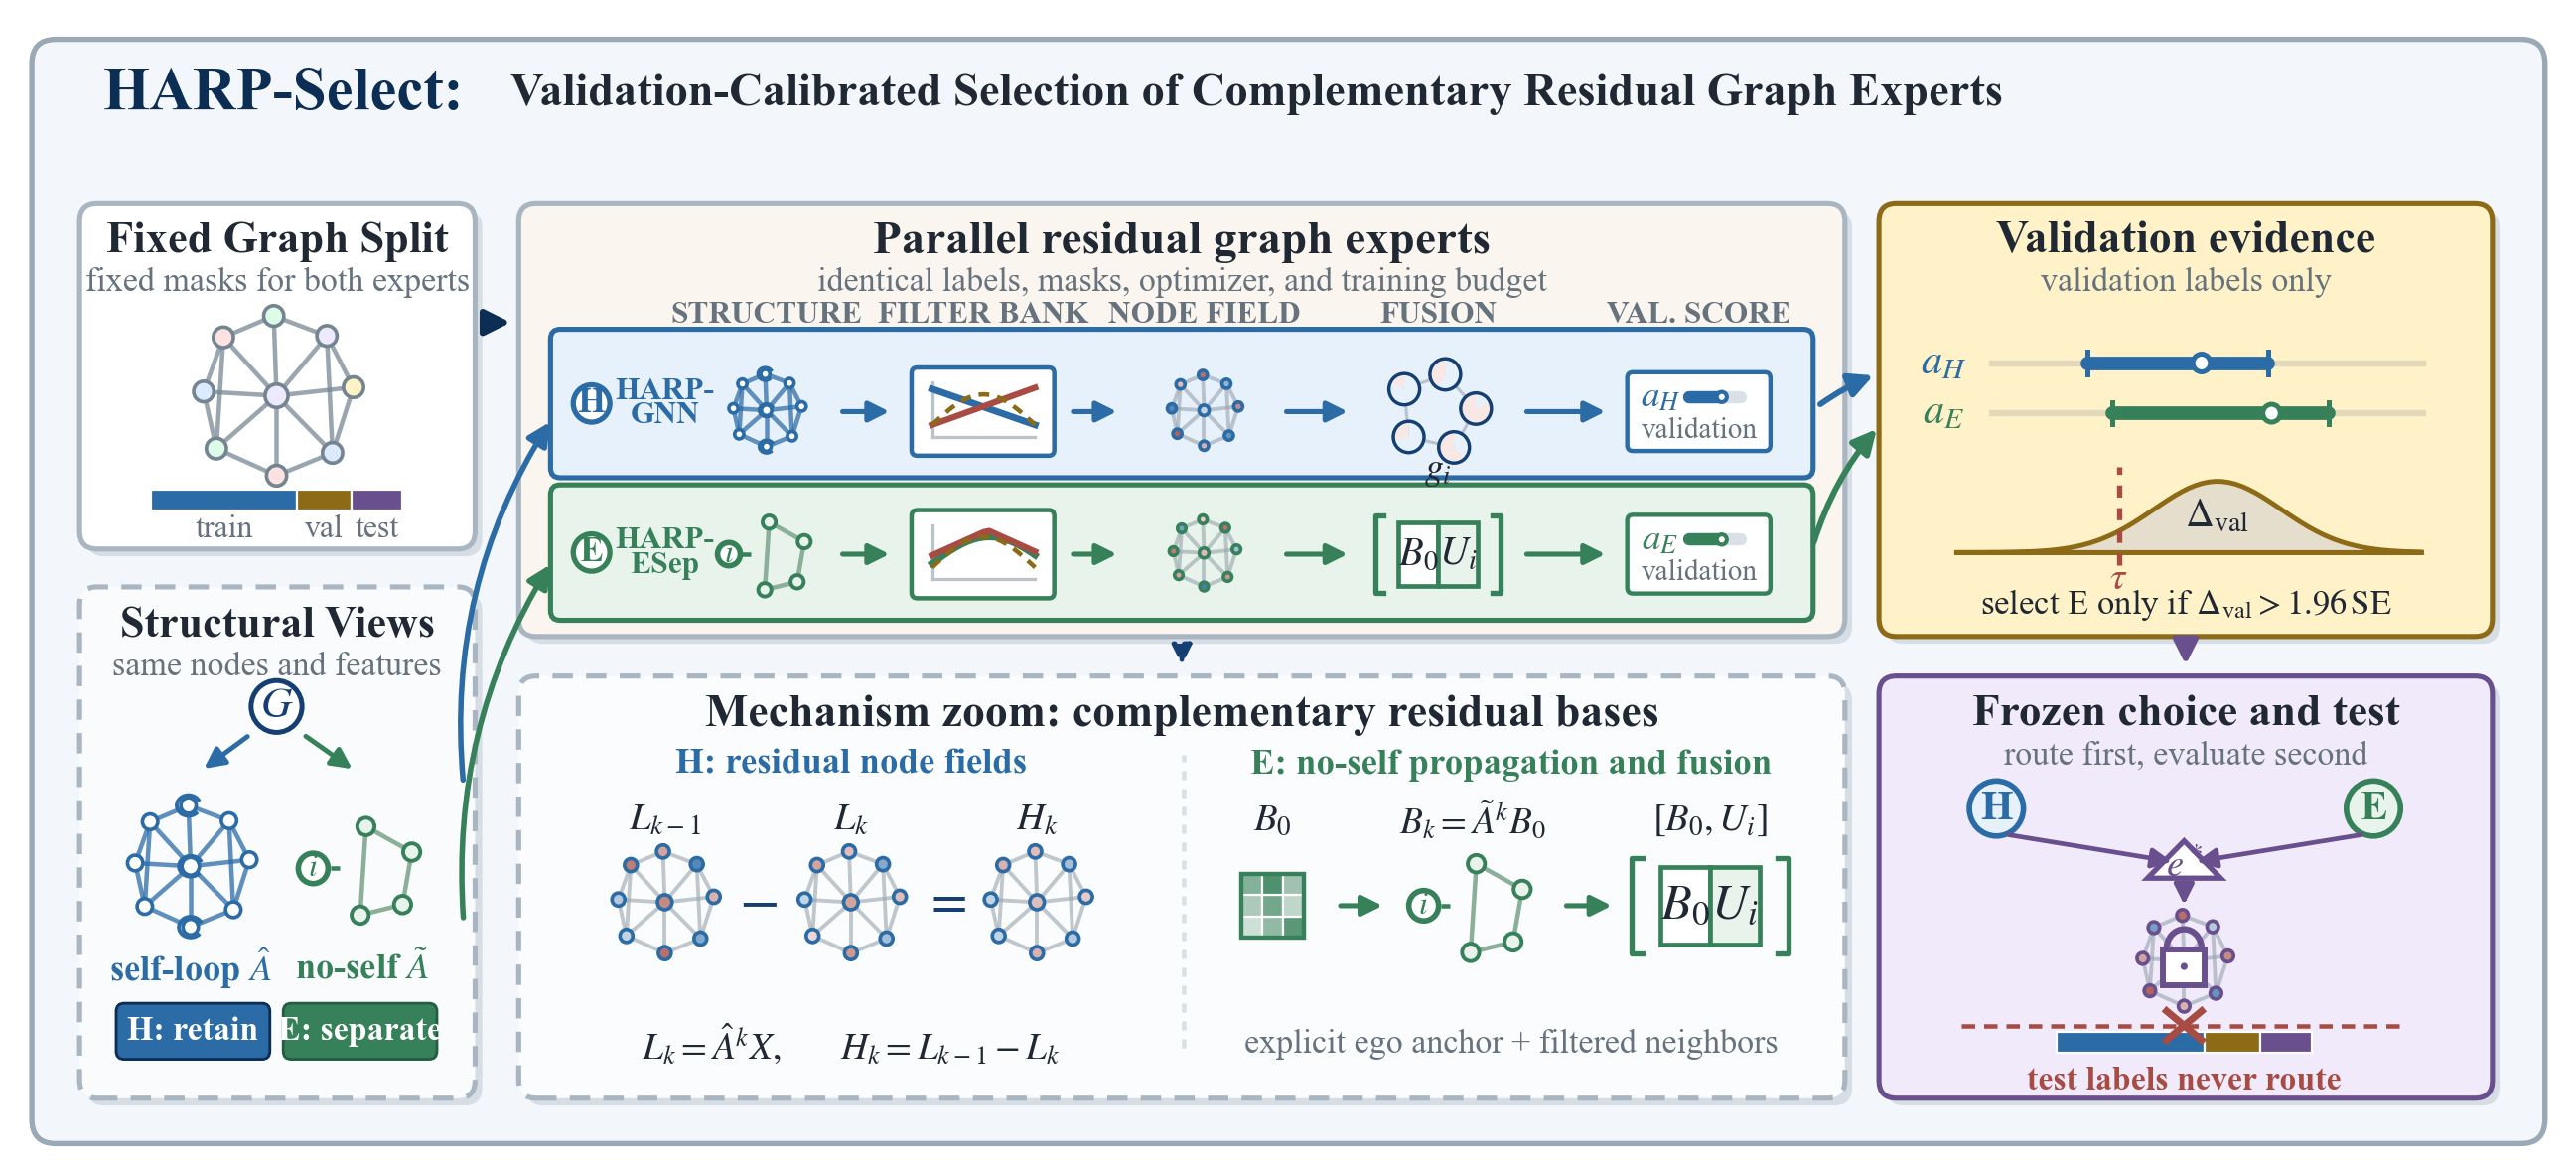
\includegraphics[width=0.78\textwidth]{figures/harp_select_framework.png}
\caption{\method{} trains two experts, records validation evidence, and freezes the branch decision before test evaluation.}
\end{figure}

\begin{figure}[H]
\centering
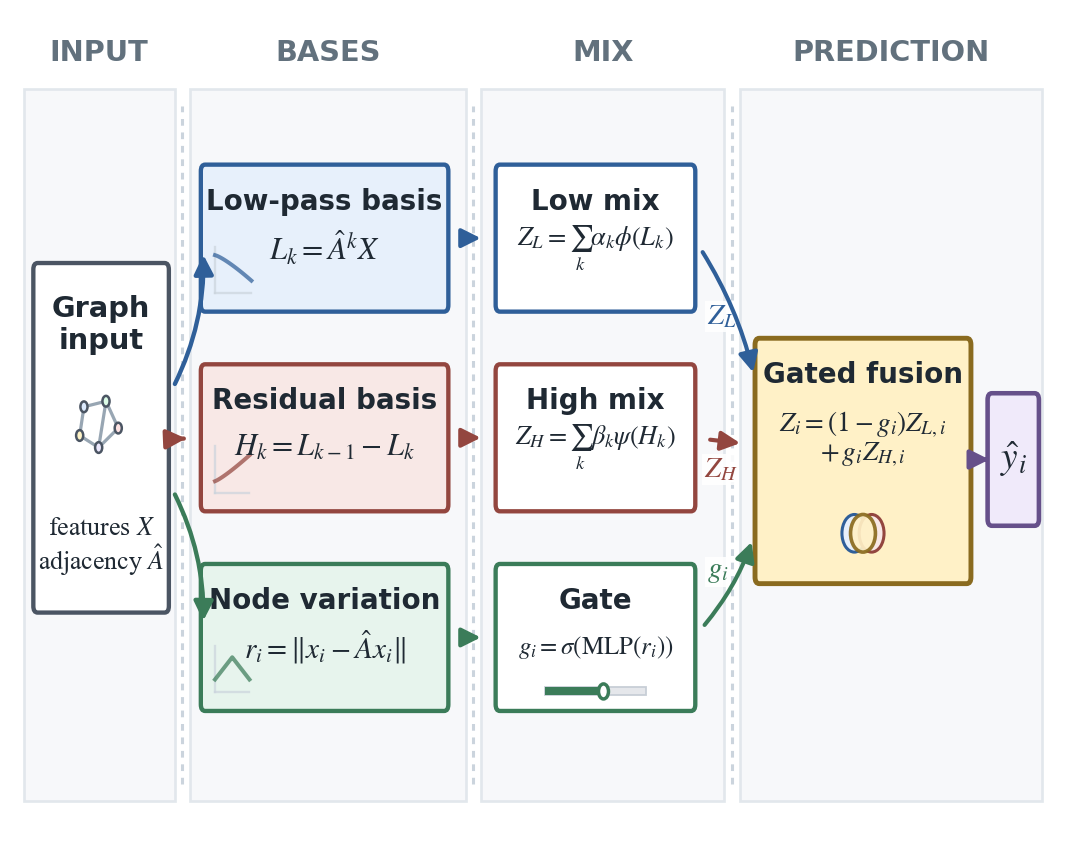
\includegraphics[width=0.78\textwidth]{figures/harp_framework.png}
\caption{Internal residual polynomial block used by the self-loop expert.}
\end{figure}

\clearpage
\section{Reproducibility Checklist for Reported Numbers}

The following scripts are the minimal checks for the numbers reported in the
main paper and this supplement:
\begin{verbatim}
python scripts\verify_implementation.py
python scripts\verify_manuscript_integrity.py
python scripts\verify_reported_results.py
python scripts\verify_top_conference_claims.py
python scripts\verify_anonymous_artifact.py --root .
\end{verbatim}

The full packaging check additionally validates the official PDF, checklist,
source package, supplementary artifact, synchronized packed sources, and LaTeX
logs:
\begin{verbatim}
python scripts\verify_submission_readiness.py
\end{verbatim}

\section{Result Coverage Audit}

\begin{table}[H]
\centering
\caption{Config/result coverage audit. Each row must be complete before a result is treated as reported evidence.}
\resizebox{\textwidth}{!}{%
\begin{tabular}{llrrrrr}
\toprule
Config & Status & Expected & Observed & Missing & Extra & Dup. \\
\midrule
configs\textbackslash{}ablation\_synthetic.yaml & complete & 24 & 24 & 0 & 0 & 0 \\
configs\textbackslash{}actor\_smoke.yaml & complete & 3 & 3 & 0 & 0 & 0 \\
configs\textbackslash{}cora.yaml & complete & 15 & 15 & 0 & 0 & 0 \\
configs\textbackslash{}critical\_heterophily\_baselines.yaml & complete & 160 & 160 & 0 & 0 & 0 \\
configs\textbackslash{}critical\_heterophily\_binary\_harp.yaml & complete & 40 & 40 & 0 & 0 & 0 \\
configs\textbackslash{}critical\_heterophily\_binary\_smoke.yaml & complete & 6 & 6 & 0 & 0 & 0 \\
configs\textbackslash{}critical\_heterophily\_harp.yaml & complete & 40 & 40 & 0 & 0 & 0 \\
configs\textbackslash{}critical\_heterophily\_smoke.yaml & complete & 4 & 4 & 0 & 0 & 0 \\
configs\textbackslash{}geom\_gcn\_harp\_esep.yaml & complete & 30 & 30 & 0 & 0 & 0 \\
configs\textbackslash{}geom\_gcn\_large.yaml & complete & 270 & 270 & 0 & 0 & 0 \\
configs\textbackslash{}geom\_gcn\_smoke.yaml & complete & 12 & 12 & 0 & 0 & 0 \\
configs\textbackslash{}harp\_x\_diagnostic.yaml & complete & 96 & 96 & 0 & 0 & 0 \\
configs\textbackslash{}planetoid\_all.yaml & complete & 75 & 75 & 0 & 0 & 0 \\
configs\textbackslash{}planetoid\_projected\_smoke.yaml & complete & 3 & 3 & 0 & 0 & 0 \\
configs\textbackslash{}planetoid\_smoke.yaml & complete & 9 & 9 & 0 & 0 & 0 \\
configs\textbackslash{}smoke.yaml & complete & 3 & 3 & 0 & 0 & 0 \\
configs\textbackslash{}synthetic\_sweep.yaml & complete & 45 & 45 & 0 & 0 & 0 \\
configs\textbackslash{}webkb.yaml & complete & 270 & 270 & 0 & 0 & 0 \\
configs\textbackslash{}webkb\_ablation.yaml & complete & 150 & 150 & 0 & 0 & 0 \\
configs\textbackslash{}webkb\_gate\_variants.yaml & complete & 120 & 120 & 0 & 0 & 0 \\
configs\textbackslash{}webkb\_h2gcn.yaml & complete & 30 & 30 & 0 & 0 & 0 \\
configs\textbackslash{}webkb\_h2gcn\_smoke.yaml & complete & 1 & 1 & 0 & 0 & 0 \\
configs\textbackslash{}webkb\_harp\_diagnostics.yaml & complete & 30 & 30 & 0 & 0 & 0 \\
configs\textbackslash{}webkb\_harp\_esep.yaml & complete & 30 & 30 & 0 & 0 & 0 \\
configs\textbackslash{}webkb\_scalar\_gate.yaml & complete & 150 & 150 & 0 & 0 & 0 \\
configs\textbackslash{}webkb\_smoke.yaml & complete & 6 & 6 & 0 & 0 & 0 \\
\bottomrule
\end{tabular}

}
\end{table}

\end{document}
